\documentclass{article}

\usepackage{graphics}
\usepackage{parskip}
%\usepackage{charter}

\title{Atari 400/800 Operating System Source Listing}
\author{Sidney~Cadot}
\date{}

\begin{document}
\maketitle
\section{Introduction}

The Atari 400/800 Operating System Source Listing (hereafter: OSSL) was originally distributed as a part of the Atari 400/800 Technical Reference Notes document.

\subsection{The Atari 400/800 Operating System}

The Atari 400 and 800 computers had a grand total of 10 kilobytes of Read Only Memory (ROM), residing at addresses \$D800-\$FFFF in the 6502 memory space.

\begin{table}
\begin{center}
\begin{tabular}{|l|l|l|}
\hline
address range & size & content                 \\
\hline
D800--DFFF    & 2 kB & Floating Point routines \\
E000--E3FF    & 1 kB & Character Bitmaps       \\
E400--FFFF    & 7 kB & Operating System        \\
\hline
\end{tabular}
\caption{A map of the Atari~400/800 ROM}
\end{center}
\end{table}

\begin{table}
\begin{center}
\begin{tabular}{|l|l|l|l|}
\hline
1--15   & 15 & n/a                                                                                     & Label definitions             \\
16--29  & 14 & E456--E458, E46E--E470, E4A6--E6D4, 0014--0014 (0)                                      & Central Input/Output (CIO)    \\
30--37  &  8 & E912--E914, E45C--E464, E46B--E46D, E480--E4A5, 900C--9020, E6D5--E90A, 0014--0014 (39) & Interrupt Handling            \\
38--60  & 23 & E459--E45B, E465--E467, E468--E46A, E48A--E48F, E944--EDE7, 0014--0014 (2)              & Serial Bus Input/Output (SIO) \\
61--63  &  3 & E450--E455, EDEA--EE77, 0014--0014 (0)                                                  & Disk Device Handler           \\
64--68  &  5 & E430--E43F, EE78--EF40, 0014--0014 (0)                                                  & Printer Device Handler        \\
69--77  &  9 & E440--E44F, E47A--E47C, E47D--E47F, EF41--F0E2, 0014--0014 (0)                          & Cassette Device handler       \\
78--90  & 13 & E471--E479, 9000--900B, F0E3--F3E3, 0014--0014 (0)                                      & Monitor                       \\
91--128 & 38 & E400--E40F, E410--E41F, E420--E42F, E488--E489, F3E4--FFF7, 0014--0014 (0)              & Display Handler (Keyboard / Screen / Editor Device Driver) \\
\hline
\end{tabular}
\caption{A map of the Atari~400/800 ROM}
\end{center}
\end{table}

9000--900B MONITOR
900C--9020 INTERRUPTS

E400--E40F DISPLAY        [EDITRV] device handler entry point for E: device
E410--E41F DISPLAY        [SCRENV] device handler entry point for S: device
E420--E42F DISPLAY        [KEYBDV] device handler entry point for K: device
E430--E43F PRINTER        [PRINTV] device handler entry point for P: device
E440--E44F CASSETTE       [CASETV] device handler entry point for C: device
E450--E452 DISK           [      ] jump vector to DINIT
E453--E455 DISK           [      ] jump vector to DSKIF
E456--E458 CIO
E459--E45B SIO            [SIOV]   jump vector to SIO
E45C--E45E INTERRUPTS     [SETVBV] jump vector to SETVBL
E45F--E461 INTERRUPTS     [      ] jump vector to SYSVBL
E462--E464 INTERRUPTS     [      ] jump vector to XITVBL
E465--E467 SIO            [SIOINV] jump vector to SIOINT
E468--E46A SIO            [SENEV]  jump vector to SENDEN
E46B--E46D INTERRUPTS
E46E--E470 CIO
E471--E473 MONITOR        [BLKBDV] jump vector to SIGNON
E474--E476 MONITOR        [WARMSV] jump vector to RESET
E477--E479 MONITOR        [COLSV]  jump vector to PWRUP
E47A--E47C CASSETTE       [RBLOKV] jump vector to RBLOK
E47D--E47F CASSETTE       [CSOPIV] jump vector to OPINP
E480--E481
E488--E489 DISPLAY        interrupt vector table entry, pointing to PIRQ5
E48A--E48B SIO            interrupt vector table entry, pointing to ISRSIR
E48C--E48D SIO            interrupt vector table entry, pointing to ISRODN
E48E--E48F SIO            interrupt vector table entry, pointing to ISRTD

E4A6--E6D4 CIO (0)
E6D5--E90A INTERRUPTS (39)
E912--E914 INTERRUPTS     [     ] jump to SETVBL (for DOS 2 compatibility)

E944--EDE7 SIO (2)      [SIOORG] SIO code
EDE8--EDE9 ---          *** unassigned *** (2 bytes)
EDEA--EE77 DISK (0)     [DSKORG] Disk device handler code
EE78--EF40 PRINTER (0)  [PRNORG] Printer device handler code
EF41--F0E2 CASSETTE (0) [CASORG] Cassette device handler code
F0E3--F3E3 MONITOR (0)  [MONORG] Monitor code
F3E4--FFF7 DISPLAY (0)  [KBDORG] Display Handler Code



Addresses \$D800 through \$DFFF contain the Floating Point routines (2 kilobytes).
Addresses \$E000 through \$E3FF contain the Atari character set (1 kilobyte).
Neither the Floating Point routines nor the Atari character set is documented in the OSSL.
What it does contain  is the remaining 7 kilobytes of ROM (addresses \$E400 through \$FFFF), containing the core operating system of
the early Atari 8-bit machines.

The OSSL is given as an assemply listing file, as generated from the original source code by the Microtec cross assembler.
The generation of the listing-file by the Microtec assembler introduces a few things:

\begin{itemize}
\item headers at the start of each page
\item maximum of 54 lines per page
\item line numbers
\item addresses and data bytes generated from the source
\item lines are truncated to 105 characters, which means that in a few places, comments are not shown in their entirity.
\end{itemize}

\section{Makefile}

\begin{figure}
\resizebox{4in}{!}{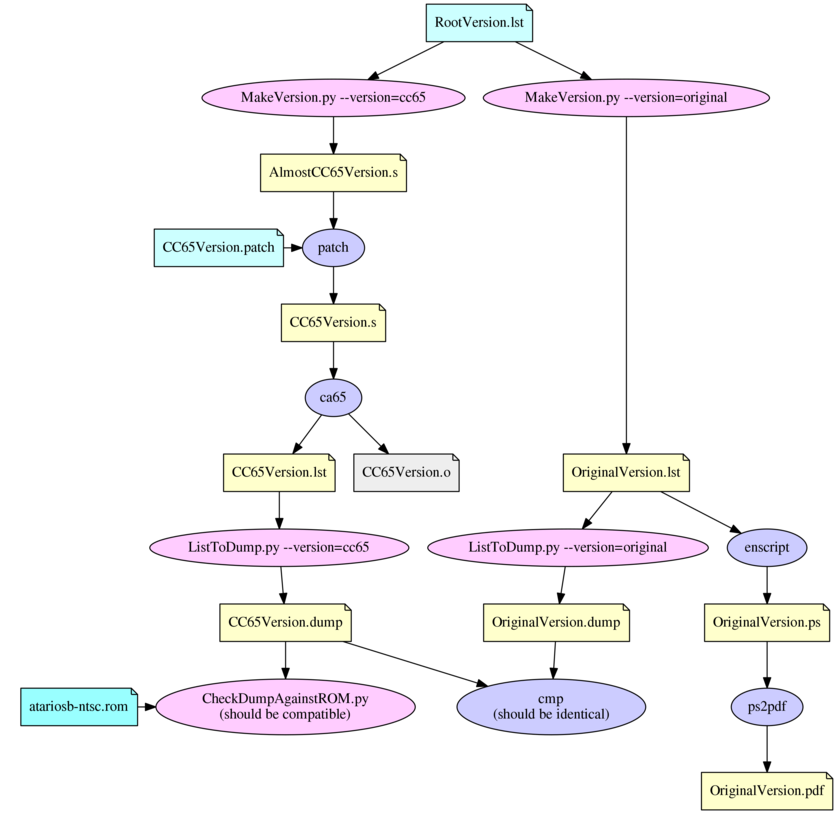
\includegraphics{DependencyGraph.pdf}}
\caption{Dependency~Graph}
\label{fig:graph}
\end{figure}

\subsection{Prerequisites}

% enscript
% patch

\subsection{Targets}

See Figure~\ref{fig:graph}.


See Figure~\ref{fig:graph}.
\end{document}
